% XeLaTeXでコンパイルしてください(他だとエラー起こすはず)
% 警告表示が出ると思うけど、PDFは生成されます(最後まで警告を無くすことが出来なかった)

\documentclass[a4paper,12pt]{bxjsreport}
\usepackage{url}
\usepackage{diagbox}
\usepackage{fontspec}
\usepackage{zxjatype}
\usepackage{caption}
\usepackage[backend=biber,style=numeric,sorting=none]{biblatex} %biblatex用
\addbibresource{bibliography.bib} %biblatex用
\setjamainfont{ipam.ttf}
\setjasansfont{ipag.ttf}
\setjamonofont{ipag.ttf}

\usepackage{amsmath,amssymb,amsfonts}
\usepackage{bm}
\usepackage{siunitx}
\usepackage[dvipdfmx]{hyperref,graphicx}
\usepackage{pxjahyper}
\hypersetup{
	colorlinks=false, % リンクに色をつけない設定
	bookmarks=true, % 以下ブックマークに関する設定
	bookmarksnumbered=true,
	pdfborder={0 0 0},
	bookmarkstype=toc
}

\usepackage{remreset}
\makeatletter
	\@removefromreset{figure}{chapter}
	\def\thefigure{\arabic{figure}}
	\@removefromreset{table}{chapter}
	\def\thetable{\arabic{table}}
	\@removefromreset{equation}{chapter}
	\def\theequation{\arabic{equation}}
\makeatother

%chapterのフォントサイズ変更
\makeatletter%%
\def\@makechapterhead#1{\hbox{}%
  \vskip-1\Cvs
  {\parindent\z@
%  \reset@font\LARGE\bfseries
  % 太字の変更はここ  
  \normalfont\huge\sffamily\gtfamily%%
  \ifnum \c@secnumdepth >\m@ne
     \setlength\@tempdima{\linewidth}%
     \vtop{\hsize\@tempdima%
         \@chapapp\thechapter\@chappos\mbox{\ \ }%
     #1}%
  \else
     #1\relax
  \fi}\nobreak\vskip1\Cvs}
\makeatother%%


%schapterのフォントサイズ変更
\makeatletter%%
\def\@makeschapterhead#1{\hbox{}%
  \vskip-1\Cvs
  {\parindent \z@ 
  \raggedright\normalfont\huge\bfseries% 左揃え
    \interlinepenalty\@M
    \huge\headfont #1\par\nobreak
    \vskip1\Cvs}}
\makeatother%%

\title{修士論文\\[1cm]ホゲホゲに関する研究\\[1cm]\\A Study on  hogehoge}
\author{〇〇大学院情報科学研究科\\〇〇専攻\\〇〇研究室\\言語 太郎\\[0.3cm]}
\date{令和〇年2月}

\begin{document}
\maketitle

% 目次
\setcounter{tocdepth}{3}
\tableofcontents

%%%%%%%%%%%%%%%%%%%%%%%%%%%%%%%%%%%%%%%%%%%%%%%%
%%%  本文
%%%%%%%%%%%%%%%%%%%%%%%%%%%%%%%%%%%%%%%%%%%%%%%
% 余白の小さなsectionとsubsectionを定義
% \newcommand{\mychapter}[1]{\vspace{-1pt}\chapter{序論}}
\chapter{序論}
\section{研究背景}
研究背景を書こう

研究背景を書こう

\begin{itemize}
\item 箇条書き1
\item 箇条書き2
\item 箇条書き3
\end{itemize}

\section{研究目的}
\label{sec:1.2}
本研究の目的を以下に列挙する.(ここの書き方は色々あります、列挙しなくても良いです)

\begin{enumerate}
\renewcommand{\labelenumi}{(\alph{enumi})}
\item 本研究の目的1
\item 本研究の目的2
\item 本研究の目的3
\end{enumerate}

目的1
次に,目的2
最後に目的3

\section{本論文の構成}
本論文では評価実験を通して提案手法の有効性を述べる.以下第2章では,関連研究について述べる.
第3章では,○について述べる.
第4章では,○について述べる.
第5章では,○について述べる.
第6章では,評価実験の方法と結果について述べる.
第7章では,考察について述べる.
第8章では,本研究のまとめについて述べる.
\chapter{関連研究}
\section{○に関する関連研究}
\label{sec:2.1}
Naguriら\cite{naguri}の研究が挙げられる.
hogehoge

\section{○○に関する関連研究}
\label{sec:2.2}
hogehogeなアプローチとして様々な手法が報告されている.

Chiuら\cite{chiu1}は○○した.

\begin{figure}[h]
 \centering
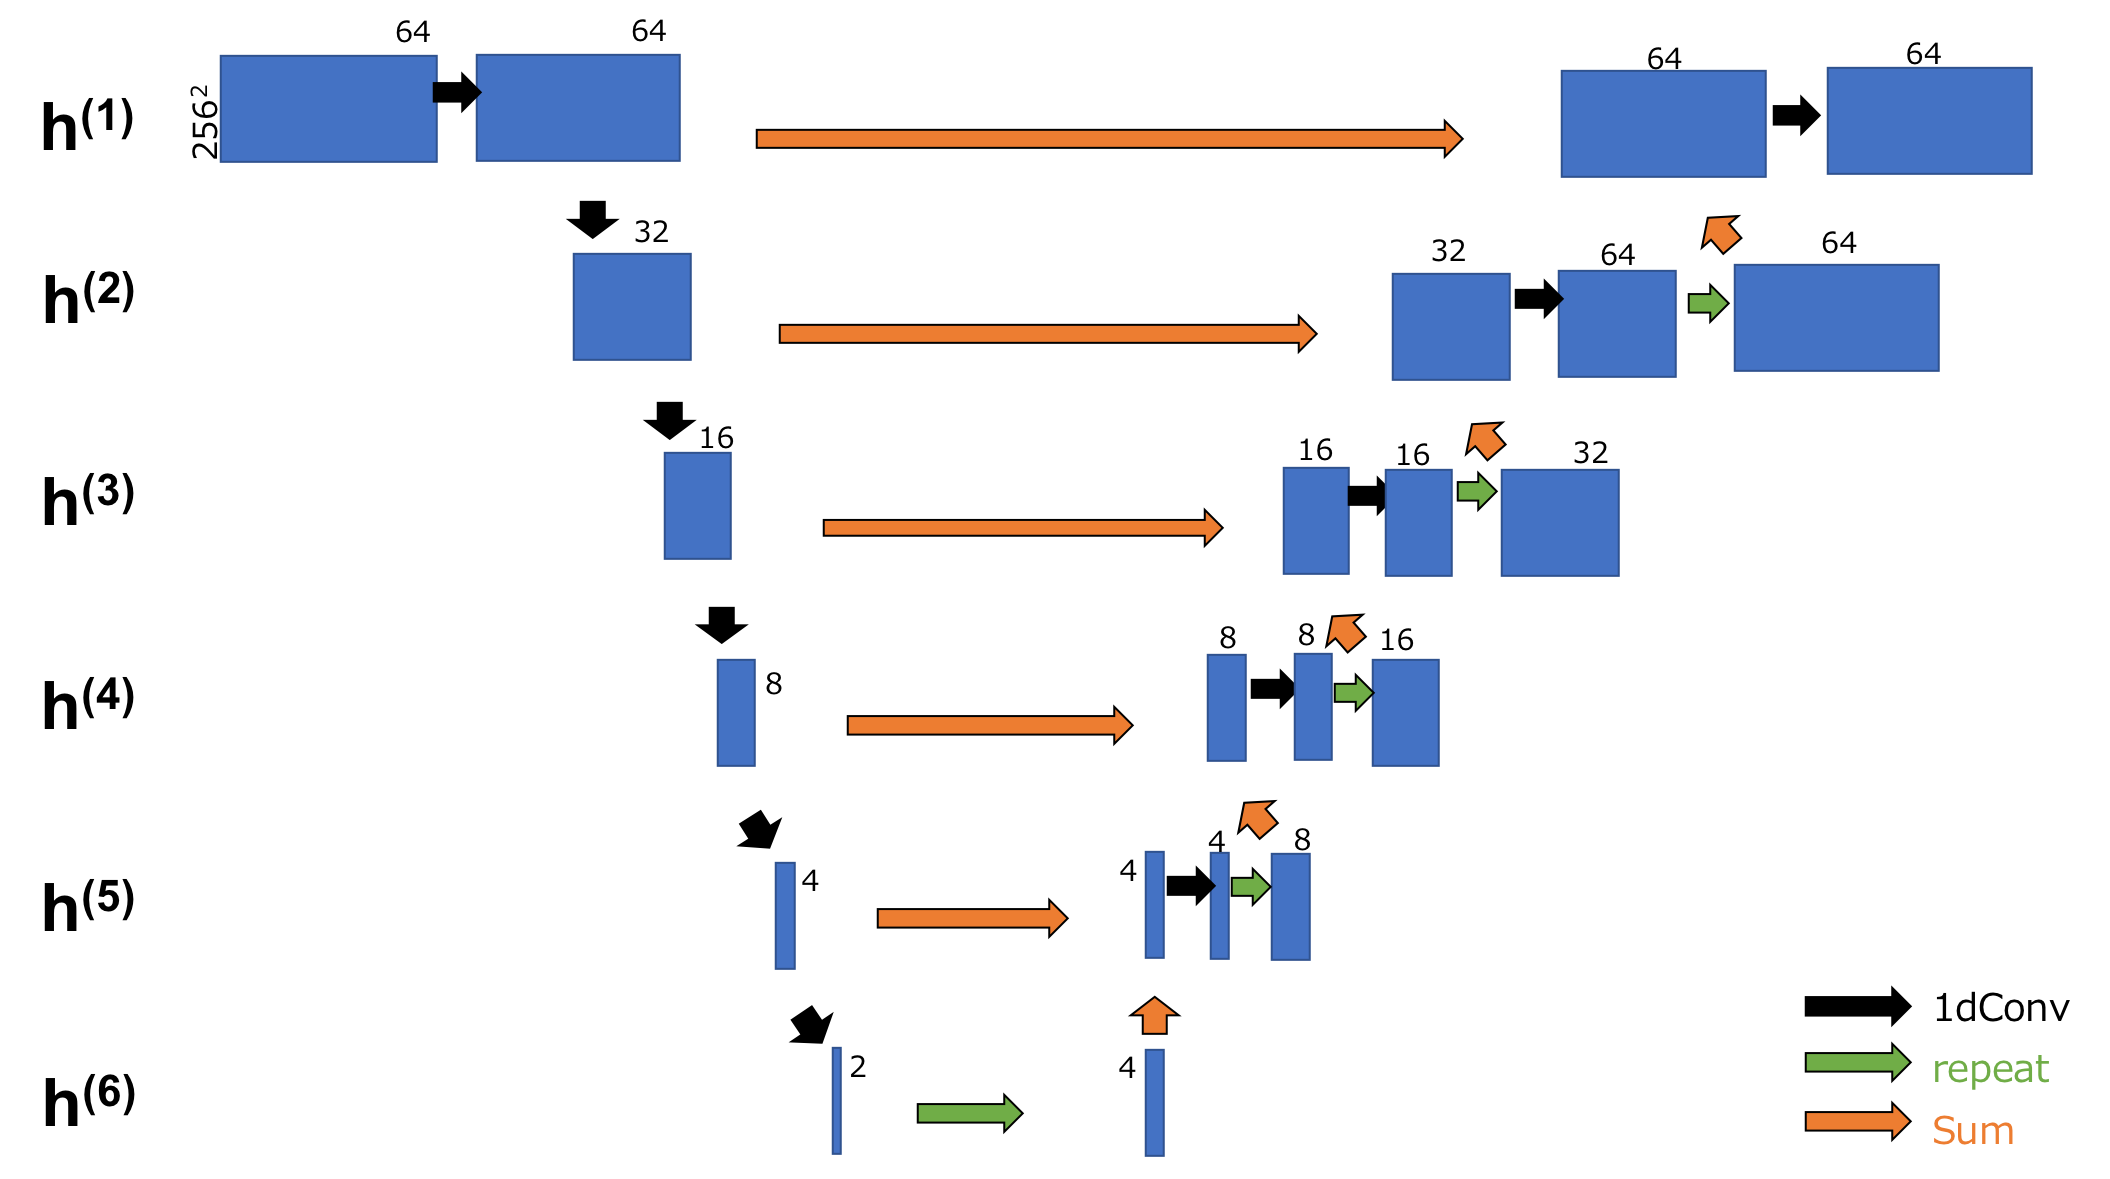
\includegraphics[keepaspectratio,width=103mm,height=77mm]{fig/net_example.png}
\caption{ネットワークの構造}
\label{fig:unet}
\end{figure}

\section{○○の応用研究}
\label{sec:2.3}
○○の応用研究として鈴木ら\cite{suzuki}の研究を紹介する.

\chapter[提案手法]{提案手法(改行時のインデントを揃\\\hspace*{2.48cm}えたければ、hspaceを使おう。)}
\section{〇〇ネットワーク}
\label{sec:4.2}
\subsection{〇〇の概要}
\label{sub:4.2.1}
\textbf{\ref{sec:3.2}}節で述べたように従来のデータセットは,音声とそれに付随するモーションであった.
レスト判定手法によって推定されたフェーズラベルを加えて,データセットを三つ組にした.
ジェスチャフェーズとレストフェーズのフェーズラベルの数を表\ref{tb:example}に示す.

\begin{table}[ht] 
\caption{表を作る} 
\label{tb:example}
\hbox to\hsize{\hfil
\begin{tabular}{c|c}\hline
ex1 & ex2 \\\hline\hline
120,962 & 130,489 \\\hline
\end{tabular}\hfil}
\end{table}

\section{〇〇処理}
\label{sec:4.3}
\subsection{従来手法での課題点}
\label{sub:4.3.1}
従来手法のネットワークから出力された〇〇は〇〇が起こった.
そこで,〇〇した.

\subsection{〇〇処理の概要}
\label{sub:4.3.2}
hogehoge

\subsection{予備実験}
\label{sub:4.3.3}

\begin{align}
hogehoge = \frac{1}{N\times64} \sum_{t=0}^N\sum_{i=0}^{64} (||\bar{x}_{t,i} -x_{t,i}||_2)
\label{eq:hogehoge}
\end{align}

ここで,$N$はhogehoge

式(\ref{eq:hogehoge})のように求められる.

\subsection{予備実験の結果}
\label{sub:4.3.4}
hogehoge
\chapter{評価実験}
\section{実験方法}
本研究では,〇〇を定量的に評価する.

hogehoge

\section{実験結果}
表\textbf{\ref{tb:example6}}に実験結果を示す.

\begin{table}[h]
\caption{評価実験の結果} 
\label{tb:example6}
\scalebox{1}[1]{
\hbox to\hsize{\hfil
\begin{tabular}{c|c|c}\hline
手法 & hogehoge1 & hogehoge2\\\hline\hline
従来手法\cite{hasegawa} & 8.618 & 0.432\\\hline
提案手法 & \textbf{8.263} & \textbf{0.511}\\\hline
\end{tabular}\hfil}}
\end{table}

hogehoge


\chapter{結果}
結果
\chapter{考察}
考察
\chapter{まとめ}
まとめ
\chapter*{謝辞}
\addcontentsline{toc}{chapter}{謝辞}

本研究を行うにあたり,研究全般における子細なご指導,ご協力を頂きました,
〇〇大学大学院情報科学研究科〇〇専攻〇〇学講座〇〇研究室,〇〇教授に深謝いたします.
\\[0.5cm]
本研究を行うにあたり,研究全般における子細なご指導,ご協力を頂きました,〇〇に深謝いたします.
\\[0.5cm]
ご多忙の中,快く副査をお引き受けくださいました,〇〇教授に深謝いたします.
\\[0.7cm]
ご多忙の中,快く副査をお引き受けくださいました,〇〇教授に 深謝いたします.
\\[0.7cm]
著者の研究期間中,数多くので協力をいただきました,本研究室の皆様に心から感謝いたします.

\cleardoublepage
\phantomsection
\addcontentsline{toc}{chapter}{参考文献}
\printbibliography[title=参考文献]  
\makeatletter
\def\@biblabel#1{(#1)}
\makeatother

% \renewcommand{\refname}{XXXXXXXX}
\renewcommand{\bibname}{研究業績}
% \renewcommand{\biblabel}[1]{#1)}
\begin{thebibliography}{99}
\setcounter{enumiv}{100}
\setlength{\labelsep}{1.0mm}
\bibitem{test1}
 test1, 教授名:“〇〇の考察”, 平成〇〇年度〇〇連合大会. 〇〇, pp. 220–221.
\bibitem{test2}
 test1, 教授名:“〇〇の考察”, 平成〇〇年度〇〇連合大会. 〇〇, pp. 220–221.
\bibitem{test3}
 test1, 教授名:“〇〇の考察”, 平成〇〇年度〇〇連合大会. 〇〇, pp. 220–221.
\end{thebibliography}

\end{document}